% This must be in the first 5 lines to tell arXiv to use pdfLaTeX, which is strongly recommended.
\pdfoutput=1
% In particular, the hyperref package requires pdfLaTeX in order to break URLs across lines.

\documentclass[11pt]{article}

% Remove the "review" option to generate the final version.
\usepackage[review]{ACL2023}

% Standard package includes
\usepackage{times}
\usepackage{latexsym}

% For proper rendering and hyphenation of words containing Latin characters (including in bib files)
\usepackage[T1]{fontenc}
% For Vietnamese characters
% \usepackage[T5]{fontenc}
% See https://www.latex-project.org/help/documentation/encguide.pdf for other character sets

% This assumes your files are encoded as UTF8
\usepackage[utf8]{inputenc}

% This is not strictly necessary, and may be commented out.
% However, it will improve the layout of the manuscript,
% and will typically save some space.
\usepackage{microtype}

% \usepackage{ctex}
% This is also not strictly necessary, and may be commented out.
% However, it will improve the aesthetics of text in
% the typewriter font.
\usepackage{inconsolata}

\usepackage{graphicx}

\usepackage{booktabs} 
\usepackage{multirow} 
\usepackage{amsmath} 
\usepackage{amssymb}
\usepackage{tikz}
\usepackage{pgfplots}
\usepackage{pgf-pie}
\usepackage{subfigure}

\definecolor{category1}{RGB}{255,153,136}
\definecolor{category2}{RGB}{247,196,127}
\definecolor{category3}{RGB}{255,227,148}
\pgfplotsset{compat=1.18} 
% If the title and author information does not fit in the area allocated, uncomment the following
%
%\setlength\titlebox{<dim>}
%
% and set <dim> to something 5cm or larger.

\title{The Music Maestro or The Musically Challenged, A Massive Music Evaluation Benchmark for Large Language Models}

% Author information can be set in various styles:
% For several authors from the same institution:
% \author{Author 1 \and ... \and Author n \\
%         Address line \\ ... \\ Address line}
% if the names do not fit well on one line use
%         Author 1 \\ {\bf Author 2} \\ ... \\ {\bf Author n} \\
% For authors from different institutions:
% \author{Author 1 \\ Address line \\  ... \\ Address line
%         \And  ... \And
%         Author n \\ Address line \\ ... \\ Address line}
% To start a seperate ``row'' of authors use \AND, as in
% \author{Author 1 \\ Address line \\  ... \\ Address line
%         \AND
%         Author 2 \\ Address line \\ ... \\ Address line \And
%         Author 3 \\ Address line \\ ... \\ Address line}

\author{First Author \\
  Affiliation / Address line 1 \\
  Affiliation / Address line 2 \\
  Affiliation / Address line 3 \\
  \texttt{email@domain} \\\And
  Second Author \\
  Affiliation / Address line 1 \\
  Affiliation / Address line 2 \\
  Affiliation / Address line 3 \\
  \texttt{email@domain} \\}

\begin{document}
% \maketitle
% \begin{abstract}
% Benchmark plays a pivotal role in assessing the advancements of large language models (LLMs). While numerous benchmarks have been proposed to evaluate LLMs' capabilities, there is a notable absence of a dedicated benchmark for assessing their musical abilities. To address this gap, we present ZIQI-Eval, a comprehensive and large-scale music benchmark specifically designed to evaluate the music-related capabilities of LLMs.
% ZIQI-Eval encompasses a wide range of questions, covering 10 major categories and 56 subcategories, resulting in over 14,000 meticulously curated data entries. By leveraging ZIQI-Eval, we conduct a comprehensive evaluation over 16 LLMs to evaluate and analyze LLMs' performance in the domain of music.
% Results indicate that only GPT-4 is capable of effectively understanding and generating music, achieving an average F1 of 58.68, suggesting that there is ample room for improvement in existing LLMs.
% With ZIQI-Eval, we aim to provide a standardized and robust evaluation framework that facilitates a comprehensive assessment of LLMs' music-related abilities.
% \end{abstract}

% \section{Introduction}
% In recent years, large language models (LLMs) have made significant advancements, revolutionizing various natural language processing tasks. 
% These models have showcased their proficiency in tasks such as accessing and reasoning about world knowledge. 

% Benchmark evaluation has played a crucial role in assessing and quantifying the performance of LLMs across different domains.
% Traditional benchmarks tailored to particular tasks such as coding~\citep{program}, reading comprehension~\citep{multispanqa}, and mathematical reasoning~\citep{cobbe2021training}, in light of the advancements made by LLMs, are increasingly regarded as inadequate for assessing their comprehensive capabilities. Consequently, there has been a surge in the emergence of more comprehensive benchmarks~\citep{liang2022holistic,srivastava2022beyond}. 

% However, both the traditional and comprehensive benchmarks have failed to adequately address the musical capability of large language models. Music is an essential part of human life and culture, and assessing LLMs' comprehension and generation of music presents a unique and challenging task. This oversight emphasizes the necessity for a comprehensive evaluation framework specifically designed to capture the nuances of the musical domain.
% % However, despite the progress made in benchmarking LLMs, there remains a significant gap in evaluating their musical abilities. Music is an essential part of human life and culture, and assessing LLMs' understanding and generation of music presents a unique and challenging task. 

% % To bridge this gap, 
% Therefore, we present ZIQI-Eval, an extensive and comprehensive music benchmark specifically crafted to assess the music-related abilities of LLMs. ZIQI-Eval comprises a diverse range of questions, systematically organized into 10 major categories and 56 subcategories. These categories cover various aspects of music, including music theory, composition, genres, instruments, and historical context. 
% In addition, this music benchmark actively contributes to the recognition of female music composers. By incorporating valuable content from these composers, it rectifies the gender disparity prevalent in historical literature, fostering advancement and inclusivity within the realm of music scholarship.
% With over 14,000 carefully crafted data entries, ZIQI-Eval provides a rich and extensive resource for evaluating LLMs' comprehension and generation of music-related content.

% Utilizing ZIQI-Eval, we carry out a comprehensive experiment over 16 LLMs, comprising API-based models and open-source models, to evaluate the performance of LLMs in the realm of music.
% Specifically, we fed music knowledge or the first half of a musical score, along with four options, into LLMs to assess their ability to select the correct option and provide meaningful explanations. 
% With an average F1 of just 58.68, even the top-performing model, GPT-4, falls short in demonstrating comprehensive music understanding and generation capabilities. 
% This observation not only exposes the overlooked aspect of music in LLMs but also emphasizes the significance of ZIQI-Eval in bridging this gap and tackling the inherent challenges associated with it.
% % Our goal was to provide a standardized and robust evaluation framework that facilitates a comprehensive assessment of LLMs' music-related abilities. This framework enables researchers and developers to benchmark their models, compare their results, and track progress in the field of music generation and understanding within the context of large language models.
% % Through the development and utilization of ZIQI-Eval, we aim to contribute to the advancement of research and development in the field of music and language models. By establishing a dedicated benchmark for assessing LLMs' musical abilities, we hope to foster innovation, encourage collaboration, and drive improvements in music-related applications powered by large language models.

% In summary, our main contributions are as follows:
% \begin{itemize}
% \item We find that existing evaluations of the capabilities of large models have overlooked their musical abilities. Therefore, we propose ZIQI-Eval benchmark, a manually curated, large-scale, and comprehensive benchmark for evaluating music-related capabilities. It consists of 10 major categories and 56 subcategories, encompassing over 14,000 data entries.
% \item We conduct evaluations on the music comprehension and music generation capabilities of 16 LLMs and find that almost all of them struggled to understand music effectively, let alone generate it. 
% % We plan to construct a multimodal benchmark for evaluating the music-related capabilities of LLMs in the future.
% \item We explore the issue of bias in LLMs' music capabilities, focusing on gender bias, racial bias, and region bias. Analysis indicates that over 35\% of LLMs exhibit biases, with region bias being the most severe. Moreover, LLMs showing one type of bias are likely to have other types of biases as well.
% \end{itemize} 

% % \newpage
% % modified
% \section{Related Work}
% \paragraph{\textbf{Music Comprehension}}
% Inspired by the field of natural language processing (NLP), previous studies represented music as embedding sequences for music understanding.
% \citet{chuan} and \citet{pirhdy} partition music pieces into distinct, non-overlapping segments of fixed duration, and train embeddings for each segment.

% Later, with the development of large language models (LLMs), recent research has utilized the modeling capabilities of these models to further enhance the understanding of music.
% MidiBERT~\citep{midibert} and MusicBERT~\citep{musicbert} both utilize pre-trained BERT to tackle symbolic-domain discriminative music understanding tasks. 
% MusicBERT further designs OctupleMIDI encoding and bar-level masking strategy to enhance pre-training with symbolic music data.
% \citet{llark} extracts music-related information from an open-source music dataset and uses instruction-tuning to instruct their proposed model LLark to do music understanding, music captioning, and music reasoning. 
% NG-Midiformer~\citep{ngramtian} first processes music pieces into  sequences, followed by leveraging N-gram encoder to understand symbolic music.

% % CLaMP~\citep{clamp} retrieves symbolic music information through learning cross-modal representations between natural language and symbolic music by utilizing a RoBERTa~\citep{roberta} text encoder and a music encoder.

% \paragraph{\textbf{Music Generation}}
% Before the proliferation of LLMs, there are some other traditional methods proposed for music generation, mainly falling into three categories: neural networks, neural audio codecs, and diffusion models.

% ~\citet{gansynth},~\citet{gacela},~\citet{greshler},~\citet{lstm-gan},
% % ~\citet{mp3net},
% ~\citet{rave}
% % ,~\citet{musika} 
% employ neural network architectures such as CNNs, RNNs, or GANs to achieve music generation.
% A neural audio codec typically contains an encoder and a decoder.~\citet{musae} follows the typical structure.~\citet{harp-net} additionally employs skip connections between the corresponding pair of encoder-decoder layers to promote reconstruction performance.~\citet{bassnet} encodes the input as a distribution rather than a single value for each dimension. Some models such as Jukebox~\citep{jukebox}, AudioLM~\citep{audiolm}, and MusicLM~\citep{musiclm} further insert a vector quantizer between the encoder and the decoder to learn a discrete latent representation.
% A diffusion model iteratively adds Gaussian noise and then learns to reverse the diffusion process to construct desired data samples from the noise. ~\citet{diffwave} proposes DiffWave, a non-autoregressive model that converts the white noise signal into structured waveform through a Markov chain. 
% ~\citet{wavegrad} combines score matching and diffusion models to generate high fidelity audio samples.~\citet{diffsound},~\citet{make-an-audio}, and~\citet{audioldm} utilize latent diffusion approach to generate high-quality music.
% % ~\citet{mousai} develops a cascading latent diffusion approach, which can generate multiple minutes of high-quality stereo music from textual descriptions.

% Since the advent of LLMs, researchers gradually began to explore the application of LLMs in music domain.
% % music comprehension and generation
% AudioGen~\citep{audiogen} and MusicGen~\citep{musicgen} both use an autoregressive transformer-based decoder~\citep{transformer} that operates on the discrete audio tokens. Macaw-LLM~\citep{macawllm} incorporates visual, audio, and textual information by using an alignment module to unite multi-modal features to textual features for LLM to generate response. 
% % NExT-GPT~\citep{nextgpt} connects an LLM with multi-modal adaptors and different diffusion decoders to enable perceiving inputs and generating outputs in arbitrary combinations of text, images, videos, and audio.
% $\mathrm{M}^2$UGen~\citep{m2ugen} exploits the potential of LLM to bridge multi-modal music comprehension and generation. It utilizes LLaMA2 model to comprehend the multi-modal contextual information of the input and perform downstream tasks such as music question-answering and music generation guidance.

% \begin{figure*}[t]
%     \centering
% % \includegraphics[width=\textwidth]{figs/tasks.pdf}
% \includegraphics[width=\textwidth]{figs/tasks_1.pdf}
%     \caption{
%         ZIQI-Eval task overview.
%     }
%     \label{fig:task-overview}
% \end{figure*}

% \paragraph{\textbf{Benchmark Evaluations}}
% Benchmark evaluation plays a crucial role in assessing the development of LLMs. Previous traditional benchmarking efforts~\citep{math,commonsense} focused on evaluating certain capabilities of models in individual tasks or single-task types. However, with the advancement of LLMs, these benchmarks have become insufficient for comprehensive and accurate assessment of LLM capabilities. Consequently, researchers have proposed more comprehensive and challenging benchmarks~\citep{mmlu,cmmlu,ceval} to test whether LLMs possess general world knowledge and reasoning ability. Additionally, there are task-specific evaluations such as LawBench~\citep{lawbench} and ArcMMLU~\citep{arcmmlu}. However, whether in English or Chinese, there is currently a lack of benchmarks for evaluating the musical abilities of LLMs, despite music being an important part of human life. Therefore, we propose ZIQI-EVAL, a benchmark for evaluating the musical abilities of LLMs, to fill the gap in benchmark evaluations of LLMs' musical capabilities.

% % modified
% \section{ZIQI-Eval Benchmark}
% \subsection{Dataset Curation}
% \paragraph{\textbf{General Principle}} 
% This dataset integrates the renowned music literature database Répertoire International de Littérature Musicale (RILM), providing a broad research perspective and profound academic insights into the dataset. The inclusion of "The New Grove Dictionary of Music and Musicians" injects the essence of musical humanism into the dataset. Furthermore, dozens of domestic and foreign monographs, such as "Music in Western Civilization" by Paul Henry Lang, the availability of past exam materials from Baidu Wenku, and the advanced data processing capabilities of GPT-4~\citep{gpt-4}, collectively enhance the data integrity and reliability of the model.

%   % \begin{table}[H]
%   %   % \begin{wraptable}{r}{0.63\textwidth}
%   %       \centering
%   %       \resizebox{0.9 \columnwidth}{!}{
%   %       \begin{tabular}{lrr}
%   %       \toprule
%   %           {\bf Category} & {\bf \# Subjects} & {\bf \# Questions} \\
%   %       \midrule
%   %       \multicolumn{3}{c}{\textit{In terms of topic}}\vspace{3pt}\\
%   %            STEM  & 20 & 4495 \\
%   %            Humanities  & 11 & 2676\\
%   %            Social Science  & 10& 2845\\
%   %            Other  & 11 & 3932\\
%   %            \midrule
%   %            \multicolumn{3}{c}{\textit{In terms of difficulty level}}\vspace{3pt}\\
%   %            Middle School  & 7 & 1409 \\
%   %            High School  & 8 & 1594\\
%   %            College  & 25 & 6249\\
%   %            Professional  & 12 & 4696\\
%   %            \midrule
%   %            \multicolumn{3}{c}{\textit{In terms of split}}\vspace{3pt}\\
%   %            Dev  & 52 & 260 \\
%   %            Valid  & 52 & 1346\\
%   %            Test & 52 & 12342 \\
%   %            \midrule
%   %            Total  & 52 & 13948 \\
%   %       \bottomrule
%   %       \end{tabular}}
%   %       \vspace{3pt}
%   %       \caption{Statistics of \ck.}
%   %       \vspace{-10pt}
%   %       \label{tab:stats}
%   %   \end{table}
    
% \paragraph{\textbf{Data Statistics}}
% ZIQI-Eval dataset consists of two parts: music comprehension question bank and msuic generation question bank.

% The music comprehension question bank which is presented in the form of multiple-choice questions consists of 10 major categories and 56 subcategories, encompassing 14244 data entries. It not only includes traditional classifications such as music performance, composition theory, and world ethnic music, but also covers popular music, Western music history, Chinese music history, Chinese traditional music, music aesthetics, and music education. The topics range from popular music, rock music, blues, to female music and more. Additionally, the dataset adopts a decentralized design philosophy, fully showcasing the diversity and inclusiveness of global music cultures. 

% The music generation question bank consists of 200 questions, testing the ability of music continuation. 
% % The first half of the music are used as the question stem, and multiple musical scores that could be the second half are provided as options to LLMs. 
% Considering the difficulty in the evaluation of the generated music, the music generation questions are also presented in the form of multiple-choice questions.

% % We separately split the objective and subjective question bank into a development set, a validation set, and a test set within each subcategory. The development set comprises five examples per subcategory to promote few-shot evaluation and the validation and test set are generated in a ratio of 1:9.


% \begin{figure}[t]
%     \centering
% \includegraphics[width=\columnwidth]{figs/example.pdf}
%     \caption{
%         Examples of music comprehension and music generation test.
%     }
%     \label{fig:example}
% \end{figure}

% We conduct a comprehensive evaluation of LLMs' music capabilities across the entire dataset. It is worth mentioning that this music dataset has made positive contributions in highlighting female music composers. By including relevant content about female composers, it addresses the gender imbalance in historical literature and promotes progress and inclusivity in the music academic community. This initiative not only reflects the model's profound recognition of gender equality issues but also demonstrates its efforts in advancing the diversification of the music field.

% \subsection{Evaluation Criteria}
% The evaluation is divided into two parts: music comprehension test and music generation test. The music comprehension test aims to assess the LLMs' music comprehension abilities, specifically their understanding of music harmony, melody, and rhythm. The music generation test, on the other hand, seeks to evaluate the LLMs' capacities for music generation, namely their ability to generate music across diverse styles and genres.

% \paragraph{\textbf{Music Comprehension Test}}
% We turn the music-related knowledge into the question stem and provide them with options to LLMs, making LLMs to choose the right answer. For example, as shown in Figure~\ref{fig:example}, take ``What is the milestone representative work of Impressionistic orchestral music?'' as the stem,  ``The Sea'', ``Prelude to the Afternoon of a Faun'', ``Pelléas et Mélisande'', and ``Clair de Lune'' as the options, we examine whether LLMs can select the right answer ``Prelude to the Afternoon of a Faun''.

% \paragraph{\textbf{Music Generation Test}}
% % Given that most LLMs can only accept textual inputs, we utilize ABC notation to convert the musical scores of audio into a textual format, which serves as the input for LLMs.

% % % ABC notation represents musical notes, rhythms, and other musical elements using plain text characters. It encodes music into two parts: header and body. The first header is the reference number and the other headers are title T, time signature M, default note length L, key K, etc.  The body mainly includes notes, bar lines and so on. Letters from A to G, and z are usually used to represent the corresponding notes and rests. For example, as shown in Figure~\ref{fig:abc}, "X:1" is the header of which 1 is the reference number and the rest content is the body.

% % The first half of the music are used as the question stem, and multiple musical scores that could be the second half are provided as options to LLMs. LLMs then choose the most likely continuation fragment, thereby assessing their music continuation ability.
% Given that most LLMs can only accept textual inputs, we utilize ABC notation to convert the musical scores of audio into a textual format, which serves as the input for LLMs.
% We partition the sheet music written in ABC notation into two segments. The initial segment serves as the question, while the subsequent segment presents four alternative options, also in ABC notation, for the potential continuation of the composition. 
% Then we make LLMs discern the most likely continuation fragment, assessing their music continuation ability. For instance, as shown in Figure~\ref{fig:example}, we split the original score from ``AABB|ccdd|ccBB|A3:|'', and test whether LLMs have the ability to choose the most fitting option.

% % modified
% \section{Experiments}
% \subsection{Setup}
% \paragraph{\textbf{Baselines}} 
% We comprehensively assess 16 LLMs, including API-based models and open-source models. The API-based models contain GPT-4 (gpt-4-1106-preview)~\citep{gpt-4}, GPT-3.5-Turbo~\citep{chatgpt}, Claude-instant-1.2~\citep{claude}, and ERNIE-Bot~\citep{ERNIE-bot} series. The open-source models contain Aquila-7B~\citep{aquila}, Bloomz-7B~\citep{bloomz}, ChatGLM2-6B~\citep{chatglm2}, 
% % Llama~\citep{llama} series, 
% Mixtral-8x7B~\citep{mixtral}, XuanYuan-70B~\citep{xuanyuan}, Qwen~\citep{qwen} series, and Yi~\citep{yi} series.

% \begin{table*}[htb]
%  \centering
%  \renewcommand\tabcolsep{8pt} % column space
%  % \small
%  \scalebox{0.85}{
%  \begin{tabular}{lcccccccccc}
%  \toprule
%   \multirow{2}{*}{Models}  & \multicolumn{3}{c}{Music Comprehension Test} & \multicolumn{3}{c}{Music Generation Test} 
%     \\\cmidrule(lr){2-4}\cmidrule(lr){5-7}
%              & Precision & Recall (Acc.) & F1 & Precision & Recall (Acc.)& F1  \\\midrule  
% GPT-4 & 63.15 & 62.93 & 63.04 & 55.15 & 53.50 & 54.31 \\
% GPT-3.5-Turbo & 55.96 & 50.18 & 52.91 & 31.77 & 30.50 & 31.12 \\
% Claude-instant-1.2 & 64.20 & 45.86 & 53.50 & 25.13 & 25.00 & 25.06 \\
% ERNIE-Bot & 74.91 & 49.96 & 59.94 & 30.05 & 29.00 & 29.52 \\
% ERNIE-Bot-Speed & 41.81 & 31.18 & 35.72 & 42.00 & 42.00 & 42.00 \\
% ERNIE-Bot-Turbo & 50.90 & 47.88 & 49.34 & 25.50 & 25.50 & 25.50 \\
% ERNIE-Bot-8k & 53.62 & 53.17 & 53.39 & 30.11 & 26.50 & 28.19 \\
%  \midrule
% Aquila-7B & 46.57 & 29.06 & 35.79 & 22.50 & 9.00 & 12.86 \\
% Bloomz-7B & 35.11 & 31.97 & 33.47 & 29.46 & 19.00 & 23.10 \\
% ChatGLM2-6B & 65.80 & 39.82 & 49.61 & 24.80 & 15.50 & 19.08 \\
% Mixtral-8x7B & 43.58 & 43.39 & 43.49 & 31.00 & 31.00 & 31.00 \\
% XuanYuan-70B & 80.73 & 37.70 & 51.40 & 23.60 & 21.00 & 22.22 \\
%         Qwen-7B & 35.95 & 14.54 & 20.70 & 24.05 & 9.74 & 13.87 \\
%         % Qwen-7B-Chat & 37.18 & 14.42 & 20.78 & 26.09 &3.00 & 5.38 \\
%        Qwen-14B & 30.04 & 17.98 & 22.49& 23.66 & 15.50 & 18.73  \\
%     Yi-6B & 60.00& 11.06 &18.68 & 0.00 & 0.00 & 0.00\\
%         Yi-34B &  32.24& 16.76 & 22.06& 12.12 & 2.00 & 3.43 \\
%     \bottomrule
%  \end{tabular}
%  }
%  \caption{Main results(\%) of the Music Comprehension Test and Music Generation Test in ZIQI-Eval. Segment 1: API-based models; Segment 2: Open-source models. 
%  % The evaluation of GPT-4/GPT-3.5-Turbo/Claude-instant-1 on objective questions is temporarily unavailable due to budget constraints.
%  }
%  \label{tab:mainres}
%  \vspace{1mm}
% \end{table*}

% % \paragraph{\textbf{Metrics}}
% % We use three metrics, namely Precision, Recall, and Accuracy, to demonstrate different aspects of LLMs' music ability.
% % \textbf{Precision} We use a regular expression $R$, namely $r'[ABCD]'$, to match the answer and consider the first uppercase letter $\in  \left \{ \text{`A'}, \text{`B'}, \text{`C'}, \text{`D'} \right \} $ matched as the response. Precision measures the accuracy of replies that can match the answer. The formula is as follows:
% % %     We calculate the probabilities that the next token predicted by LLMs belongs to each vocab token, select the probabilities that belong to the option letters and take the option which owns the highest probability as LLMs' choice. Given an input sequence $\mathbf{X} = [x_1, x_2, \ldots, x_n]$, the calculating process is as follows:
% % % \begin{gather*}
% % % \mathbf{P} = p_\theta \left ( \mathbf{X} \right ) = \left[p_{x_2},p_{x_3}, \ldots, p_{x_{n+1}}  \right] \\
% % % \mathbf{Q} = Softmax(\mathbf{P}) \\
% % % q_{op} = Softmax(\mathbf{Q}_{op}), op \in \left \{ \text{`A'}, \text{`B'}, \text{`C'}, \text{`D'} \right \} \\
% % % \hat{y} = argmax\left (q_{op}  \right) \\
% % % Accuracy = \frac{\sum_{i=1}^{N} \mathbb{I}\left ( \hat{y_i} = y_i \right ) }{N}
% % % \label{eq:1}
% % % \end{gather*}
% % % where $p_\theta \left ( \cdot  \right )$ is the LLM; $\mathbf{P} \in \mathcal{R}^{b\times n \times C} $, $b$ is the batch size and $C$ is the vocab size; $N$ is the total number of questions; $\mathbb{I}\left ( \cdot  \right )$ is the indicator function.
% % \begin{gather*}
% % \tilde{X} = G\left ( X \right ) \\
% % \hat{y} = R\left ( \tilde{X} \right )  \\
% % Accuracy = \frac{\sum_{i=1}^{N} \mathbb{I}\left ( \hat{y_i} = y_i \right ) }{N}
% % \label{eq:1}
% % \end{gather*}
% % where $G$ is the LLM generation process, $\tilde{X}$ is the generated string, $R\left ( \cdot  \right ) $ is applying the regular expression for answer retrieval, $\hat{y}$ is the predicted answer, $N$ is the number of replies that can match an answer, and $\mathbb{I}\left ( \cdot  \right )$ is the indicator function.
% % \textbf{Recall} LLMs' output may lack meaningful content or be completely unrelated to the input. To consider the effectiveness of the LLMs' output, we use a Recall score. When the output of a question is meaningful and relevant to the question, the Recall score is 1; otherwise, it is 0. The calculation formula is as follows:
% % \begin{equation*}
% %    Recall = \frac{Num(\mathcal{V})}{N} 
% % \end{equation*}
% % where $\mathcal{V}$ is the valid output set, and $Num\left ( \cdot  \right ) $ is the number of $\mathcal{V}$.

% %  \textbf{F1} We calculate the F1 score as the Accuracy score for LLMs:
% %     % We multiply the accuracy score and the recall score to calculate the accuracy score, thereby measuring the overall music abilities of LLMs:
% % \begin{equation*}
% %     Accuracy=\frac{2\ast Precision\ast Recall}{Precision + Recall} 
% % \end{equation*}
% % % \begin{equation*}
% % %     accuracy = 100 \ast recall \ast Accuracy
% % % \end{equation*}
% \paragraph{\textbf{Metrics}}
% We use a regular expression $R$, namely $r'[ABCD]'$, to match the answer and consider the first uppercase letter $\in  \left \{ \text{`A'}, \text{`B'}, \text{`C'}, \text{`D'} \right \} $ matched as the response.
% We define Accuracy (Acc.) as the proportion of correctly answered questions among all questions. Precision is the proportion of correctly answered questions among the questions predicted as A/B/C/D. Recall is the proportion of correctly answered questions among the total number of questions that should be answered as A/B/C/D. In this case, the total number of questions that should be answered as A/B/C/D is actually the total number of questions, so the recall metric is equivalent to the accuracy metric. F1 score is the weighted harmonic mean of precision and recall. The specific formulas for these metrics are as follows:
% \begin{gather*}
% \tilde{X} = G\left ( X \right ) \\
% \hat{y} = R\left ( \tilde{X} \right )  \\
%     Precision = \frac{\sum_{i=1}^{N} \mathbb{I}\left ( \hat{y_i} = y_i \right ) }{V} \\
%     Recall (Acc.) = \frac{\sum_{i=1}^{N} \mathbb{I}\left ( \hat{y_i} = y_i \right ) }{N} \\
%     F1 = \frac{2\ast Precision\ast Recall}{Precision + Recall} 
% \end{gather*}
% where $G$ is the LLM generation process, $\tilde{X}$ is the generated string, $R\left ( \cdot  \right ) $ is applying the regular expression for answer retrieval, $\hat{y}$ is the predicted answer, $V$ is the number of questions predicted as A/B/C/D, $N$ is the total number of the questions, and $\mathbb{I}\left ( \cdot  \right )$ is the indicator function.

% \subsection{Results}
% Table~\ref{tab:mainres} presents the main results of ZIQI-Eval. Based on the results, we can find that:

% \paragraph{\textbf{\uppercase\expandafter{\romannumeral1}.}} \textbf{Overall, the performance of all LLMs on the ZIQI-Eval benchmark is poor.} 
% % Whether it is on music comprehension questions assessing music knowledge ability or music generation questions assessing music continuation ability, LLMs behave underwhelmingly. 
% % In the music comprehension and generation test, a\% and A\% of the models respectively have a lower effective accuracy than the random selection accuracy of 25\%. Additionally, b\% and B\% of the models respectively have an accuracy that is approximately equal to 25\% (with a fluctuation of less than 1.00\%), only c\% and C\% of the models respectively have an accuracy greater than 25\%.
% % These findings suggest that the majority of LLMs lack proficiency in music ability. Even the highly advanced LLM, GPT-4, exhibits an average accuracy of merely 57.38, falling short of the minimum passing threshold of 60. This glaring discrepancy highlights the inadequate consideration given to music accuracy within current LLM models and underscores the formidable challenges posed by the ZIQI-Eval benchmark.
% In both music comprehension test and music generation test, the majority of LLMs have not surpassed the passing threshold of 60. Their accuracy rates generally hover between 30 and 50, performing only marginally better than random selection. Even the top-performing model, GPT-4, achieved accuracy rates of only 63.04 and 54.31 in the respective tests. This glaring discrepancy highlights the inadequate consideration given to music abilities within current LLM models and underscores the formidable challenges posed by the ZIQI-Eval benchmark.

% \paragraph{\textbf{\uppercase\expandafter{\romannumeral2}.}} \textbf{API-based models perform better than open-source models.} In the evaluation of music comprehension test, API-based models generally exhibit higher accuracy compared to open-source models. The accuracy of API-based models is basically distributed between 50 and 70, while open-source models mostly range between 20 and 50. Only specific open-source models like XuanYuan-70B can achieve an accuracy higher than 50.

% In the evaluation of music generation questions, API-based models apparently outperform open-source models with significantly higher accuracy. The highest accuracy achieved by an API-based model is 54.31, surpassing the highest accuracy of 31.00 in open-source models.

% \paragraph{\textbf{\uppercase\expandafter{\romannumeral3}.}} \textbf{The music capabilities of LLMs are dependent but not solely on parameter size.} There is a certain degree of relationship between the musical ability and parameter size of LLM models within the same series, while the musical ability of LLM models from different series is not strongly correlated with parameter size.
% % It can be observed that the Llama series models show an increase in accuracy as the parameter size increases, except for a decrease in performance from 13B to 70B parameters in the evaluation of objective questions. 

% The Qwen series and Yi series LLMs consistently show improvements in both music comprehension and generation F1.
% % Different LLM models, such as Bloomz with 7.1B parameters, achieve an accuracy of 47.33 in music comprehension test, while XuanYuan with 70B parameters has an accuracy of only 41.72. There is a difference in accuracy between Aquila-7B and Boom, which have similar parameter sizes.
% Contrary to expectations, the model with significantly different parameter sizes, ChatGLM2-6B and Yi-34B, exhibits higher F1 in music comprehension for the ChatGLM2-6B model, surpassing Yi-34B by 27.55. Even among models with similar parameter sizes, there can be considerable differences in performance. For example, the Yi-6B model achieves a music comprehension F1 of only 18.68, while ChatGLM2-6B achieves an F1 of 49.61, resulting in a significant difference of 30.93 between the two F1 scores.

% \paragraph{\textbf{\uppercase\expandafter{\romannumeral4}.}} \textbf{The instruction-following abilities of LLMs are not directly linked to their music capabilities.} The precision scores of LLMs are strongly correlated with their instruction-following abilities. However, a strong instruction-following capability does not necessarily indicate strong musical capabilities in LLMs. Some LLMs may score highly in terms of precision, but they struggle to effectively comprehend and generate music. Yi-6B serves as a clear example where the comprehension precision score reaches 60.00, but the F1 is only equivalent to 18.68.

% \paragraph{\textbf{\uppercase\expandafter{\romannumeral5}.}} \textbf{The music generation capabilities of LLMs are in need of improvement.} Even though some LLMs demonstrate a decent understanding of music, their music generation capabilities still have room for improvement. In general, the F1 for music generation test in LLMs are lower compared to music comprehension test. The difference can be quite significant, such as ERNIE-Bot-8k, where the score for music comprehension test is higher by 25.20 compared to music generation test.

% \begin{table}[htb]
%  \centering
%  \renewcommand\tabcolsep{2pt} % column space
%  \scalebox{0.85}{
%      \begin{tabular}{lcccc}
%      \toprule
%       % Models & Female & Black & Region \\0.01
%       \multirow{2}{*}{Models}  & \multirow{2}{*}{Female} & \multirow{2}{*}{Black} & \multicolumn{2}{c}{Region} \\
%         \cmidrule(lr){4-5}
%                  & & & European & Other \\
%      \midrule  
%      GPT-4                   & 66.67   & 85.71   & 60.00   & 64.97   \\
% GPT-3.5-turbo           & 47.37   & 64.15   & 45.09   & 52.49   \\
% Claude-instant-1.2      & 45.16   & 50.00   & 88.89   & 53.13   \\
% ERNIE-Bot & 49.04 & 78.57 & 49.96& 32.48\\
% ERNIE-Bot-Speed         & 59.09   & 14.29   & 75.28   & 31.61   \\
% ERNIE-Bot-Turbo         & 48.26   & 58.18   & 64.80   & 50.03   \\
% ERNIE-Bot-8k            & 48.95   & 75.00   & 65.92   & 39.49   \\
%      \midrule
% Aquila-7B               & 26.31   & 29.27   & 13.25   & 17.45   \\
% Bloomz-7B             & 37.87   & 56.60   & 28.90   & 32.94   \\
% ChatGLM2-6B             & 25.88   & 48.89   & 23.84   & 30.95   \\
% Mixtral-8x7B            & 47.32   & 67.86   & 40.00   & 48.76   \\
% XuanYuan-70B &38.35 & 70.54& 37.70  &38.17\\
% Qwen-7B & 23.40 & 20.51 & 26.67 & 18.11 \\
%             % Qwen-7B-Chat & 19.56 & 23.81 & 18.46 & 17.93\\
%             Qwen-14B & 23.45 & 21.74 &16.30 & 25.22\\
%            Yi-6B &33.26 & 21.62 & 40.00 & 24.39\\
%            Yi-34B & 20.63 & 15.00 & 19.85 & 23.29 \\
%      \midrule
%             Average &40.06   & 48.62   & 43.53   & 36.47\\
%      \bottomrule
%      \end{tabular}
%     }
%  \caption{Results(\%) of Female Music F1, Black African Music F1, F1 Of European Music and other regions' music in World Ethnic Music. \textit{Female} stands for Female Music F1, \textit{Black} stands for Black African Music F1, and \textit{Region} stands for the F1 of LLMs regarding World Ethnic Music, beneath which \textit{European} stands for European Music F1 and \textit{Other} stands for other regions' music F1.}
%  \label{tab:ablation}
%  \vspace{1mm}
% \end{table}

% \begin{table}[htb]
%  \centering
%  \renewcommand\tabcolsep{5pt} % column space
%  \scalebox{1.0}{
%  \begin{tabular}{lcc}
%  \toprule
%   Models & Female & Black \\
%  \midrule  
%         GPT-4  & & \\
%         GPT-3.5-Turbo & & \\
%         % Claude-instant-1 & -& -&- & 25.00 & 99.50 & 24.88 \\
%         ERNIE-Bot & 49.04 & 78.57 \\
%         ERNIE-Bot-Speed & 58.85 & 14.29  \\
%         ERNIE-Bot-Turbo & 40.41 & 32.14  \\
%         ERNIE-Bot-8k & 46.61 & 64.29  \\
%  \midrule
%         Aquila-7B & 19.76 & 21.43 \\
%         Bloomz-7.1B & 33.63 & 50.00  \\
%         ChatGLM2-6B & 19.47 & 39.29  \\
%         % Llama-7B & 28.91 & 28.57  \\
%         % Llama-13B & 35.10 & 42.86  \\
%         % Llama-70B & 36.50 & 38.39  \\
%         Mixtral &46.90 &67.86  \\
%         Qwen-7B-Chat & 58.96 & 75.00  \\
%         XuanYuan-70B &38.35 & 70.54 \\
%         Yi-6B &100.00 & 64.29  \\
%  \midrule
%         Average & 43.75 & 49.11 \\
%  \bottomrule
%  \end{tabular}
%  }
%  \caption{Results(\%) of Female Music Accuracy and Black African Music Accuracy. \textit{Female} stands for Female Music Accuracy, and \textit{Black} stands for Black African Music Accuracy.}
%  \label{tab:ablation}
%  \vspace{1mm}
% \end{table}

% \section{Analysis}
% In addition to the overall evaluation of LLMs on the dataset, we are also interested in the models' ability for specific categories.

% Aquila-7B, Bloomz-7.1B, ChatGLM2-6B, Llama-7B, Llama-13B, Llama-70B, XuanYuan-70B
\begin{figure*}
\centering
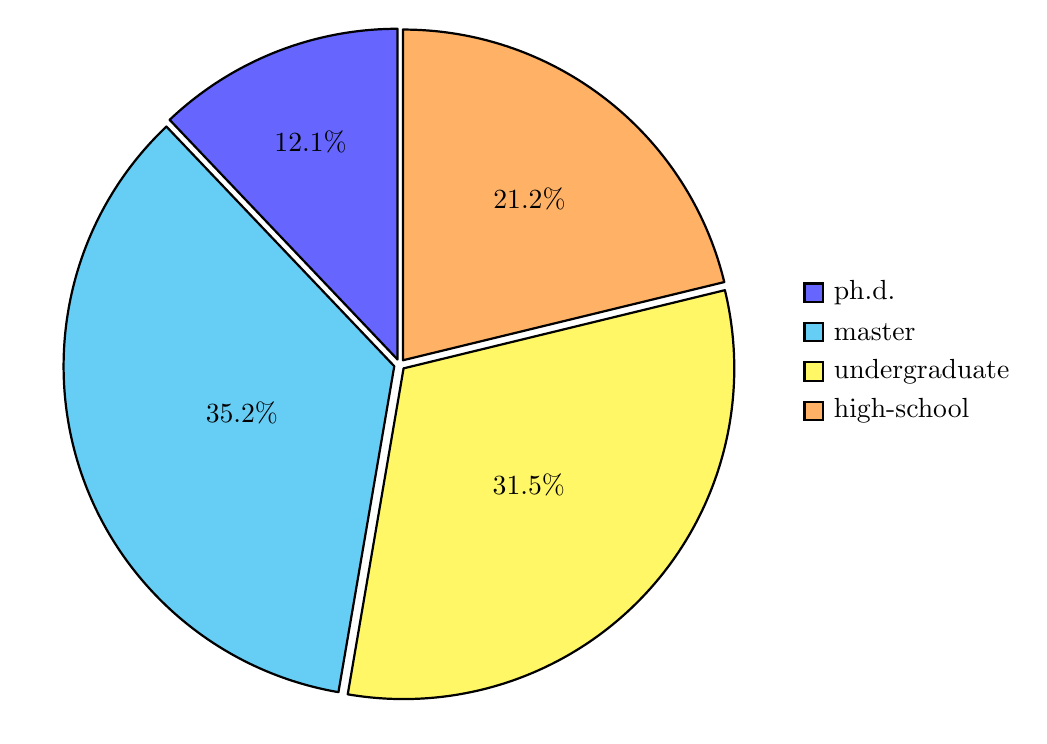
\begin{tikzpicture}[scale=0.7]
% % \pie[explode=0.1, text=legend, color={category1,category2,category3}]{20/Aquila-7B |
% % Bloomz-7.1B |
% % ChatGLM2-6B |
% % Llama-7B |
% % Llama-13B |
% % Llama-70B |
% % XuanYuan-70B, 
% % 30/ERNIE-Bot-Turbo |
% % ERNIE-Bot-8k |
% % Mixtral,
% % 50/ERNIE-Bot |
% % ERNIE-Bot-Speed |
% % Qwen-7B-Chat |
% % Yi-6B 
% % }

% % \pie[pos = {20,0}, explode=0.1, text=legend, color={category1,category2,category3}]{20/ERNIE-Bot-Speed |
% % ERNIE-Bot-Turbo |
% % Aquila-7B |
% % ChatGLM2-6B |
% % Llama-7B |
% % Llama-13B |
% % Llama-70B |, 
% % 30/Bloomz-7.1B,
% % 50/ERNIE-Bot |
% % ERNIE-Bot-8k | 
% % Mixtral |
% % Qwen-7B-Chat |
% % XuanYuan-70B |
% % Yi-6B 
% % }
% rotate = 90,
\pie[explode=0.1, text=legend, radius=6, rotate = 90]{
12.1/ph.d.,
35.2/master,
31.5/undergraduate,
21.2/high-school
}

% \pie[pos = {0,0}, explode=0.1, radius=6, rotate = 90,text=legend]{
% 59.4/Music major \& with musical background,
% 32.1/Non-music major \& without musical background,
% 8.5/Non-music major \& with some musical background
% }

% \pie[pos = {0,-14}, explode=0.1,radius=6, rotate = 90, text=inside]{37.50/unbiased, 
% 6.25/neutral,
% 56.25/biased
% }

% \pie[pos = {14,-14}, explode=0.1, radius=6, rotate = 90,text=inside]{37.50/unbiased, 
% 6.25/neutral,
% 56.25/biased
% }
\end{tikzpicture}
\caption{Depiction of of proportions in different categories. Left: gender bias. Right: racial bias.}
\label{bias}
\end{figure*}

% \begin{tikzpicture}

% % Pie chart 1
% \pie{10/A, 20/B, 30/C, 40/D}

% % Pie chart 2
% \pie[
% 	pos = {7.5,0},
% 	rotate = 90
% ]{10/A, 20/B, 30/C, 40/D}
% \label{gender-bias}
% \end{tikzpicture}

% \begin{figure*}[htb]
%   \centering
%   \setlength{\abovecaptionskip}{0cm}
%   \setlength{\belowcaptionskip}{-0.3cm} 
%   \scalebox{1.0}{
%   % \hspace{0.5in} % 两图片之间的距离
%   \subfigure[accuracy]{
%     \label{accuracy} 
%     \includegraphics[width=0.61\textwidth]{figs/model_scores_by_region-2.pdf}}
%   \subfigure[Proportion]{
%     \label{proportion} 
%     \includegraphics[width=0.41\textwidth]{figs/bias-pie.pdf}}}
%   \caption{Performance of LLMs on gender bias, racial and region bias.}
%   \label{bias} 
% \end{figure*}

% \begin{figure*}[t]
%     \centering
% \includegraphics[width=0.61\textwidth]{figs/bias.pdf}
%     \caption{
%         Performance of LLMs on gender, racial and region bias.
%     }
%     \label{fig:example}
% \end{figure*}

% \subsection{Does LLM show any bias towards questions related to women?}
% \label{gender}
% % average: 43.75
% We compare the F1 of LLMs in the female music theme with the average F1 obtained by LLMs in the female music theme to analyze whether there is bias in LLMs towards female music. We categorize LLMs into three groups: LLMs without gender bias (above the average F1), LLMs with no significant bias (deviating within a range of $\pm$5.0\% from the average F1), and LLMs with gender bias (below the average F1).

% Because we do not fine-tune LLMs, the results reflect the inherent biases of the LLMs themselves. According to the results of Table~\ref{tab:ablation}, 50.00\% of the models have no gender bias, 6.25\% of the models are neutral or have no significant bias, and 43.75\% of the models have gender bias.
% % , as shown in Figure~\ref{proportion}.
% LLMs with F1 lower than the average F1 tend to overlook relevant content related to female music themes. Yi-34B and Aquila-7B, in particular, have significantly lower scores than the average, indicating a notable gender bias issue in these two models.
% % Overall, LLMs exhibit minimal gender bias.

% \subsection{Does LLM exhibit bias toward different races?}
% We calculate the F1 of LLMs for the subtopic of Black African music, using the same partitioning method as for determining gender bias, to assess whether there is racial bias in LLMs.
% % We use the same categorization method as in Section~\ref{gender} to assess whether LLMs have racial bias.
% According to the results of Table~\ref{tab:ablation}, 50.00\% of the models have no racial bias, 12.50\% of the models are neutral or have no significant bias, and 37.50\% of the models have racial bias.
% % , as shown in Figure~\ref{proportion}.
% The F1 of ERNIE-Bot-Speed and Yi-34B are below the mean by 34.33 and 33.62 respectively, indicating a significant racial bias in these two models.
% % Overall, LLMs exhibit minimal racial bias.

% \subsection{Does LLM display bias in terms of region?}
% We seek to investigate whether LLMs are influenced by Eurocentrism, which positions Europe as the cultural and knowledge center, potentially leading to lower evaluations or neglect of contributions from non-central regions and resulting in biases against these regions. To assess the presence of region bias, we computed the F1 for the European Music subtheme within World Ethic Music, and the average F1 for other subthemes within World Ethic Music.
% Among the LLMs, 43.75\% exhibited higher F1 rates in European Music compared to other regional music, while 37.5\% of LLMs demonstrated higher F1 rates in European Music than the average F1 rate within European Music. These findings suggest that LLMs are influenced by Eurocentrism and exhibit bias towards non-central regions.
% % Most LLMs show similar F1 between European music and other regions. 
% Surprisingly, ERNIE-Bot-Speed and Claude-instant-1.2 exhibit significantly higher F1 scores in European music compared to other regions, 43.67 and 35.76 respectively, demonstrating a clear regional bias inclination.

% % done
% From Figure~\ref{fig:example}, it is evident that LLMs demonstrate similar tendencies towards gender bias, racial bias, and region bias, displaying a trend where both ends (with bias and without bias) are relatively higher, while the middle (neutral) is lower. Some LLMs have F1 scores significantly lower than the mean, such as Yi-34B with an F1 lower than the mean by over 50\%, suggesting that LLMs still have a long way to go in eliminating biases. It is worth noting that LLMs with a propensity for gender bias are likely to exhibit racial bias and region bias as well, as evidenced by models such as Aquila-7B, Qwen series, and Yi series. Consequently, it is imperative for future developments in LLMs to address biases comprehensively, not limited to gender, racial and region biases.
% % encompassing not only gender bias but also racial bias and beyond.
% % \begin{figure}
% %     \centering
% %     \includegraphics[width=1\linewidth]{figs/bias2.pdf}
% %     \caption{Enter Caption}
% %     \label{fig:enter-label}
% % \end{figure}

% % modified
% \section{Futher Analysis}
% \subsection{Phenomenon Analysis of LLMs }
% To further explore the generation capabilities of LLMs in the realm of music, we conduct an in-depth analysis of the responses provided by each model. Our findings categorize the existing LLMs into three distinct types:

% \paragraph{\textbf{\uppercase\expandafter{\romannumeral1}.}} \textbf{Lack of melodic understanding: }This type includes LLMs that demonstrate a complete lack of comprehension regarding musical notation. When faced with questions that require the continuation of a melody after a format transformation, these models predominantly resort to evasion, often responding with statements like "Unable to determine, need more information." They fail even to understand the format of the input melody. ChatGLM2-6B and Aquila-7B are prototypical examples of this type, characterized by a high frequency of evasive responses, resulting in a significantly low efficacy in their replies. A notable phenomenon is their tendency to "guess" by consistently selecting option A, leading to most responses without any analytical explanation. For instance, in the responses from ChatGLM2-6B, option A was chosen up to 60\%. Besides a preference for option A, Aquila-7B also shows a partiality towards option D.

% \paragraph{\textbf{\uppercase\expandafter{\romannumeral2}.}} \textbf{Limited appreciation, misaligned with human preferences: }A representative model in this type is ERNIE-Bot-8K. This model provides highly interpretable analyses for each option of every question, offering seemingly logical explanations concerning melody, rhythm, and pitch. However, the model's performance, with accuracy barely exceeding that of random selection, underscores the challenge of encapsulating the subjective essence of music appreciation through algorithmic processes. This discrepancy not only highlights the limitations of current AI models in understanding complex, subjective domains but also underscores the need for more sophisticated approaches that can better capture the intricacies of human preferences. 

% \paragraph{\textbf{\uppercase\expandafter{\romannumeral3}.}} \textbf{Relatively good appreciation skills: }GPT-4 stands out as a typical example of this type. Its responses consider aspects such as melodic coherence, stylistic similarity, and the seamless integration of musical structures, aligning to a certain extent with human preferences. Further analysis of the questions GPT-4 answered reveals a incorrectly strong inclination towards musical continuity. In many instances, it is observed that GPT-4 prioritized coherence, which leads to the selection of incorrect options.

% \subsection{Analysis of GPT-4}

% Taking GPT-4 as a case study, we have gained further insights into the performance of LLMs in the realm of music. The performance of GPT-4 in the domains of female music and world ethnic music indicates a commendable understanding of specific musical areas, reflecting GPT-4's focus on diversity and inclusivity.Female music and world ethnic music, each representing unique cultural and social perspectives, have shown GPT-4's extensive coverage of different cultures and musical traditions through its relatively higher scores.

% GPT-4 has demonstrated exceptional performance in the realm of popular music, achieving scores close to 90. This may be due to the abundant and accessible resources in popular music, including lyrics, genres, and artist information. The popularity and media coverage of pop music may also have facilitated the model's learning efficiency in this field.

% It has also scored high in western music history and musical performance, showcasing its capability in processing music history and practical music-making. The higher scores in western music history over all other regions suggest a certain degree of region bias.

% In the area of music aesthetics, GPT-4 scored low, revealing a significant weakness. This may be attributed to the complexity and subjectivity of music aesthetics, which might surpass the model's ability to learn from existing textual materials, indicating that there is room for improvement in the model's perception, evaluation, and theoretical analysis of music.

% Through analysis, we identify that GPT-4 tends to make errors in several distinct categories, primarily falling into three types:

% \textbf{Matching Errors:} This category encompasses questions related to musical knowledge, specifically matching-type queries, such as identifying the first Hungarian national opera or the composer of "The Song of the Red Flag". GPT-4's responses often affirmatively state incorrect options, indicating inaccuracies within its knowledge base for specific factual information.

% \textbf{Comprehension Errors:} These errors involve understanding specific musical terminologies and the relationships between certain concepts. Questions like "What function of art does edutainment refer to?"  or "What role do work songs play in labor as a genre of folk music?" exemplify where GPT-4 misinterprets multiple word meanings, leading to a misunderstanding of the intended concept. This suggests a need for improvement in GPT-4's understanding within the musical domain.

% \textbf{Reasoning Errors: }In instances where GPT-4 correctly understands the question and possesses the relevant knowledge background, errors occur during the reasoning or calculation process, resulting in incorrect conclusions. An example can be seen in questions involving the calculation of musical intervals, where GPT-4 confuses semitones and whole tones. This indicates a gap in GPT-4's ability to perform downstream tasks that require precise musical logical deductions.

% % modified
% \section{Conclusion and Future Work}
% Our research sheds light on the oversight of existing evaluations in recognizing the musical abilities of large models. To address this gap, we introduce ZIQI-Eval, a comprehensive benchmark that encompasses 10 major categories and 56 subcategories, comprising over 14,000 data entries. Notably, this benchmark also actively contributes to the acknowledgment of female music composers, rectifying the gender disparity and promoting inclusivity.
% % prevalent in historical literature and promoting inclusivity within the field of music scholarship.
% We conduct a comprehensive experiment involving 16 LLMs, including both API-based and open-source models, to assess their performance in the domain of music. The results indicate that there is significant scope for enhancing the musical capabilities of existing LLMs.
% We intend to create a multimodal benchmark to evaluate the musical expertise of LLMs in the future.
% % to foster a more comprehensive understanding and assessment of their musical prowess.
% % By continuously advancing the evaluation frameworks, we aim to foster a more comprehensive understanding and assessment of these models' musical prowess.
% % \section{Limitations}
% % Entries for the entire Anthology, followed by custom entries
% \section*{Limitations}
% Our research to date has been exclusively focused on objective questions, without delving into the study of subjective questions. One limitation of our current music benchmark is the absence of multi-modal data. While the benchmark may excel in evaluating and comparing the quality and creativity of musical compositions based on audio data alone, it fails to incorporate other essential aspects of the music experience, such as visual elements or textual information.

% \newpage
% \begin{figure}
% \centering
% \begin{minipage}{0.45\linewidth}
% \centering
% \begin{tikzpicture}
% \pie[text=legend]{50.0/Female, 6.25/, 43.75/}
% \end{tikzpicture}
% \caption{Female}
% \end{minipage}
% \hfill
% \begin{minipage}{0.45\linewidth}
% \centering
% \begin{tikzpicture}
% \pie{text=legend}{50.0/Black, 12.5/, 37.5/}
% \end{tikzpicture}
% \caption{Black}
% \end{minipage}

% \vspace{1em}

% \begin{minipage}{0.45\linewidth}
% \centering
% \begin{tikzpicture}
% \pie{text=legend}{37.5/European, 6.25/, 56.25/}
% \end{tikzpicture}
% \caption{European}
% \end{minipage}
% \hfill
% \begin{minipage}{0.45\linewidth}
% \centering
% \begin{tikzpicture}
% \pie{text=legend}{37.5/Other, 6.25/, 56.25/}
% \end{tikzpicture}
% \caption{Other}
% \end{minipage}
% \caption{Distribution of Bias}
% \end{figure}

% \bibliography{anthology, custom}
% \bibliographystyle{acl_natbib}

\appendix

% \section{Example Appendix}
% \label{sec:appendix}
% \paragraph{Prompt}
% Among the following composers, whose music creations have an impressionistic style? Option A, Debussy, Dukas, Ravel; Option B, Debussy, Dukas, Hindemith; Option C, Hindemith, Delius, Lespighi; Option D, Ravel, Hindemith, Lespighi. 请你严格按照以下格式输出:[[答案:]]解析
\end{document}
